%!TEX root = Main.tex
\documentclass[Main]{subfiles}

\begin{document}
\subsection{CO$_2$ Level Estimation} % (fold)
\label{sub:co__2_level_estimation}

	In order to give the user feedback on whether the current CO$_2$ emission level is \emph{HIGH} or \emph{LOW} you need two pieces of information.

	\begin{itemize}
		\item Data on CO$_2$ emission levels
		\item Knowledge of what constitutes a \emph{HIGH} or \emph{LOW} emission level
	\end{itemize}

	The available data is described in Section \ref{sub:c02_emission_data}.
	For this project it is elected to use the \emph{online} data, as this fits our use case best.
	Firstly, because \emph{prognosis} data about future levels are not very useful for a user, as people are unlikely to postpone the use of the elevator, even with the knowledge of any potential savings from doing so.
	Secondly, the short time nature of elevator use fits very well with the short time nature of the \emph{online} data.
 
	% subsection co__2_level_estimation (end)

	\subsubsection{Decision Making} % (fold)
	\label{sub:decision_making}

		Making a decision on whether CO$_2$ emission levels are \emph{HIGH} or \emph{LOW} requires a threshold, distinguishing the two, to be set.
		For this project a threshold of $340\ grams\ \sfrac{CO_2}{kWh}$ is set.
		This level the Danish national average from 2012, provided by Energistyrelsen \cite{Energistyrelsen:2012:Online}.

		To reduce flickering between \emph{HIGH} and \emph{LOW} with insignificant change in CO$_2$ emission levels, some hysteresis has been implemented.
		This means that the data must drop $3\ grams\ \sfrac{CO_2}{kWh}$ below the threshold to change from \emph{HIGH} to \emph{LOW}.
		Likewise the data must rise $3\ grams\ \sfrac{CO_2}{kWh}$ above the threshold to change from \emph{LOW} to \emph{HIGH}.
	
		% sub-subsection decision_making (end)


	\subsubsection{Shortcomings and Future Work} % (fold)
	\label{sub:shortcomings_and_future_work}
		We suspect that using the same global threshold for all days of the year is not the most effective method, as the general trend in CO$_2$ emissions are unlikely to be all year round.
		This would lead to long periods of either \emph{HIGH} or \emph{LOW} states.
		It is hypothesized that such monotony in level indication would lead to users ignoring the signal and go back to their normal habits.

		Comprehensive modeling of CO$_2$ emissions and user susceptibility to input is beyond the scope of this project.
		Even though, some analysis of CO$_2$ emissions trend is presented in Section \ref{sub:trends_in_co2_data} below for the sake of completeness and enabling future improvement.

		% sub-subsection shortcomings_and_future_work (end)


	\subsection{Trends in CO$_2$ Data} % (fold)
	\label{sub:trends_in_co2_data}
		
		In this section some examples of CO$_2$ emission data is presented.

		\begin{figure}[H]
			\centering 
			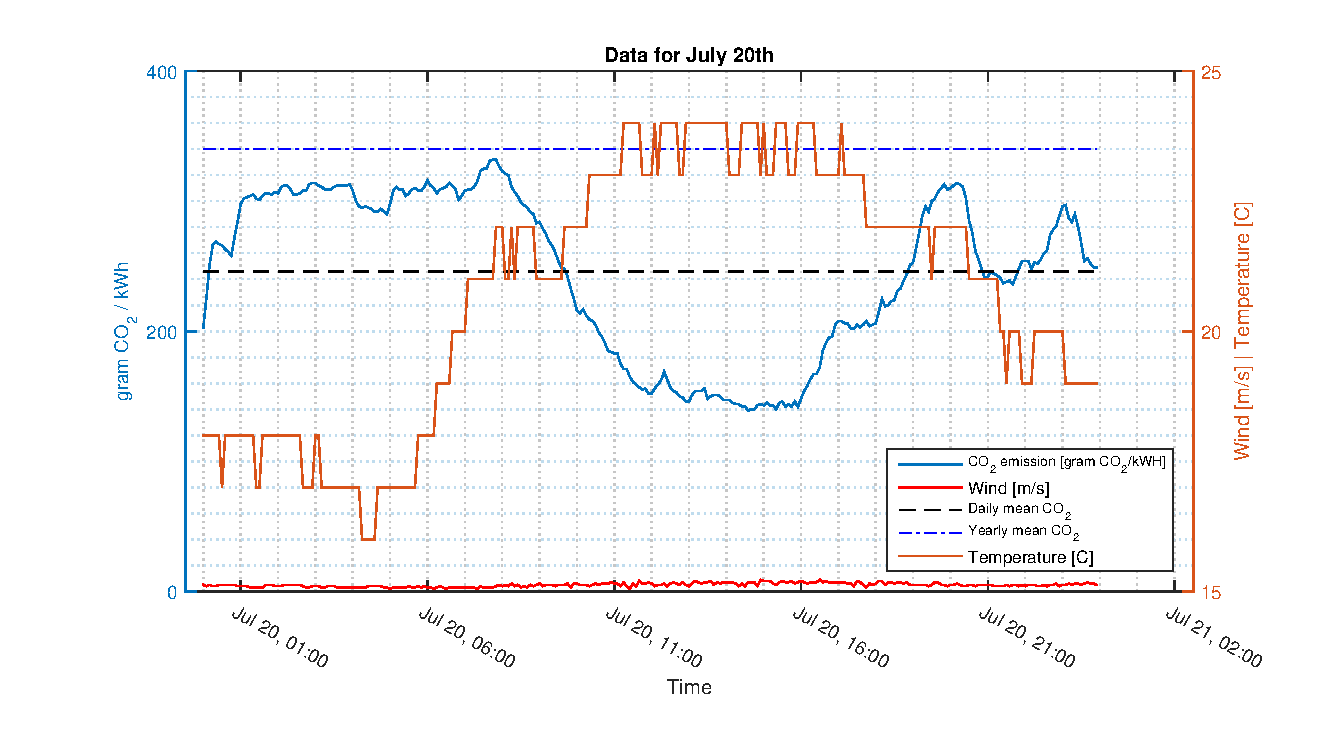
\includegraphics[width=\textwidth]{Summer.eps}
			\caption{CO$_2$ emission data for a summer day}
			\label{fig:Summer}
		\end{figure}

		Figure \ref{fig:Summer} above is a clear example of why adaptive thresholding is necessary.
		At no point during this day does the CO$_2$ emission rise above the global threshold.
		It also shows that, at least on this day, there were a strong negative correlation between temperature and CO$_2$ emission.
		The wind does not seen to fluctuate much or have much effect on CO$_2$, and hence it has been dropped from the following figures.


		\begin{figure}[H]
			\centering
			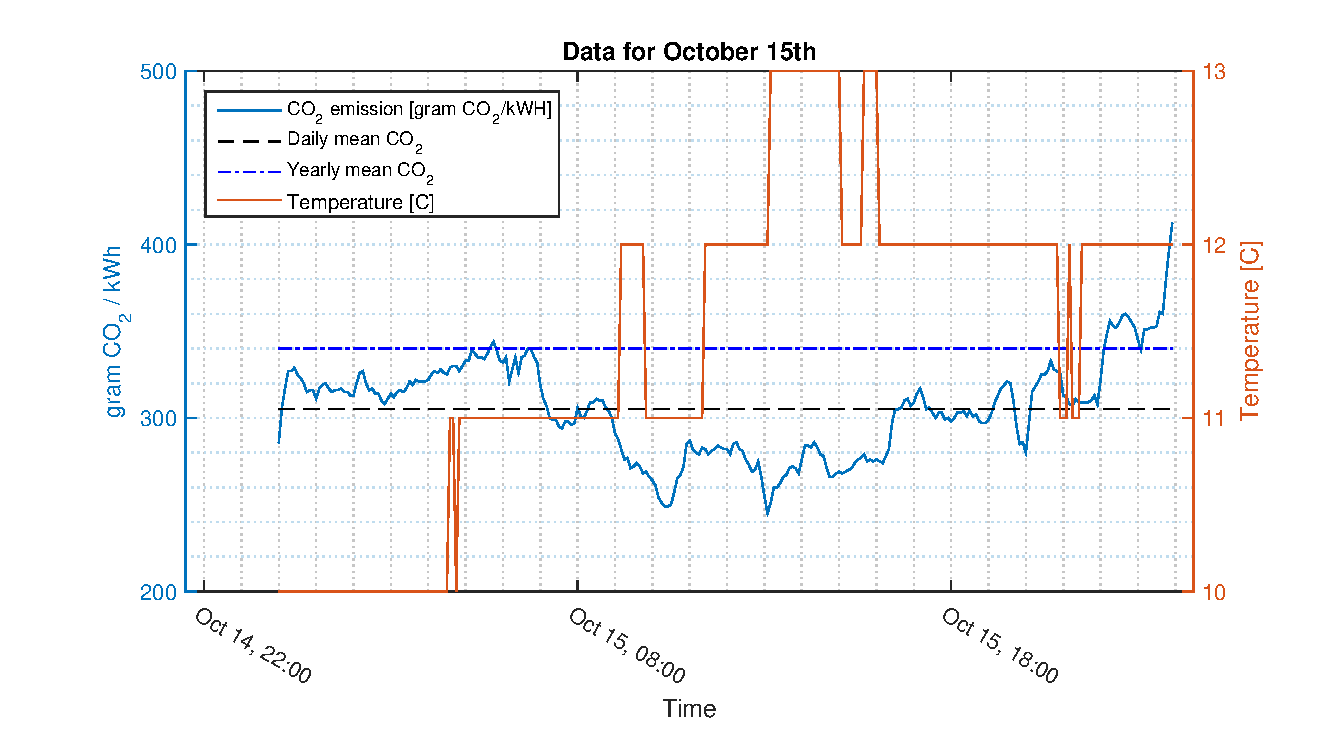
\includegraphics[width=0.9\textwidth]{Autum.eps}
			\caption{CO$_2$ emission data for an Autumn day}
			\label{fig:Autum}
		\end{figure}

		Figure \ref{fig:Autum} above show a normal autumn day. Here the CO$_2$ emission level is both above and below the threshold.


		\begin{figure}[H]
			\centering
			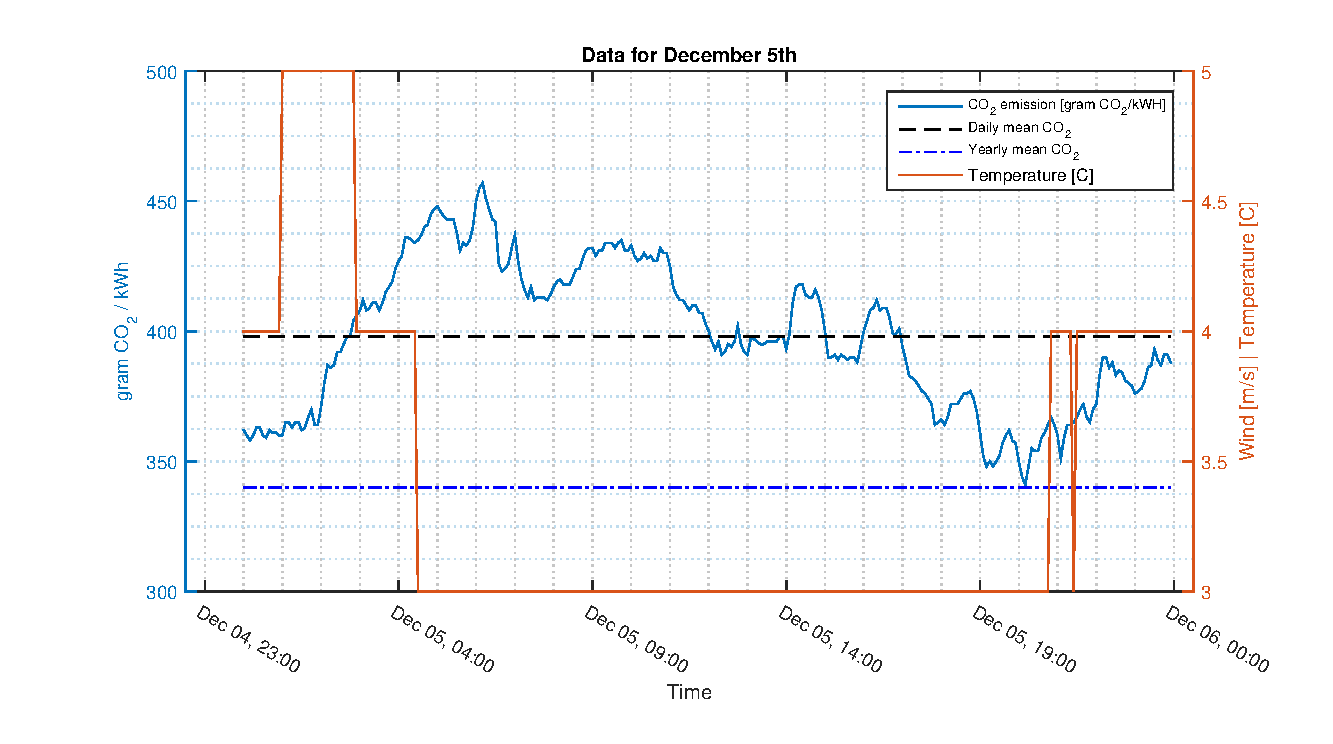
\includegraphics[width=0.9\textwidth]{Winter.eps}
			\caption{CO$_2$ emission data for a winter day}
			\label{fig:Winter}
		\end{figure}
		% subsection trends_in_co2_data (end)

		Figure \ref{fig:Winter} show a normal winter day.
		Again we see a case where the CO$_2$ emission levels fluctuate a lot during a day, but does not cross the average threshold.

		What we see in Figures \ref{fig:Summer}, \ref{fig:Autum} and \ref{fig:Winter} above, confirms our assumption of season shift and the necessity of a more complex CO$_2$ emission trends model.
		

\end{document}